\section{Dota 2}

\begin{figure}[htbp]
\begin{center}
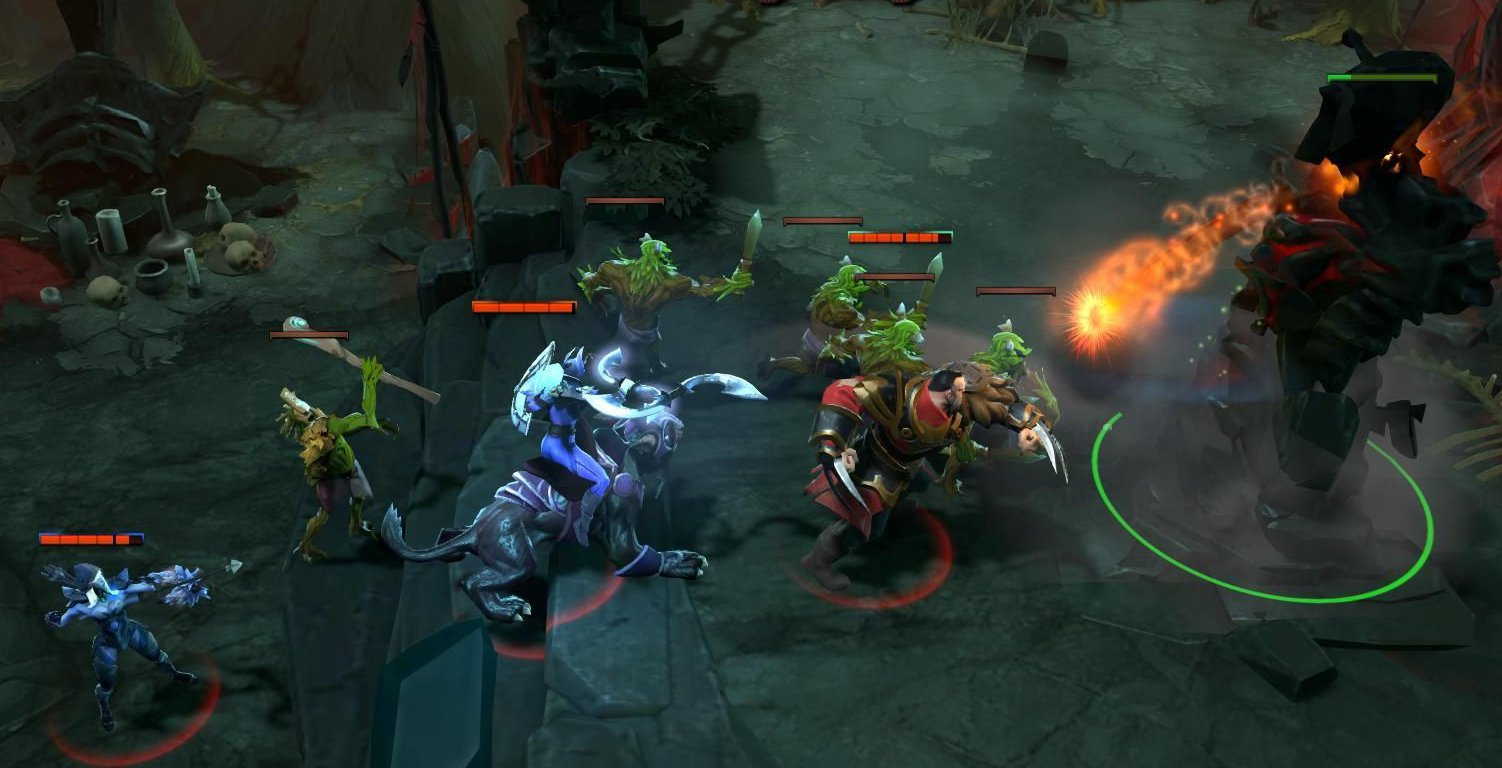
\includegraphics[width=.60\textwidth]{./imagenes/dota2.jpg}
\caption{Dota 2}
\label{Dota 2}
\end{center}
\end{figure}
Dota 2 \footnote{\url{http://dota2.com/}} es un juego creado por Valve basado en el popular mod de Warcraft 3, Defense of the Ancients. Es un juego de estrategia en equipo para ser jugado con equipos de 5 personas cada uno.
Dota 2 combina elementos de estrategia en tiempo real con perspectiva "en tercera persona", incorporando a todo ello un sistema de nivelación y jugabilidad de diversos juegos de rol como Diablo. Los jugadores asumen el papel de una unidad clasificado como un "héroe", que puede subir de nivel hasta un máximo de 25. La configuración básica de Dota 2 consiste en dos ciudades de distinta forma, cada una cuenta con una fortaleza de defensa conocida como "ancestro", situadas en los extremos opuestos de un mapa equilibrado de manera uniforme. Entre ellas hay varias regiones de conexión identificado como "caminos", que son atravesados por unidades enemigas, al tiempo que luchan contra poderosas torres defensivas a lo largo del camino. Los jugadores se dividen entre dos equipos, cada uno con hasta cinco jugadores, para competir como los principales defensores de cada Fortaleza de los Ancestros.

\subsubsection{¿Por qué es uno de mis juegos favoritos?}
\begin{itemize}
\item[Victor Cedeño] Este es un juego que requiere de comunicación y cooperación entre 5 personas para poder lograr el objetivo de vencer al otro equipo. Es muy dificil jugar solo sin la ayuda de tus compañeros. El juego tiene una gran selección de mas de 100 heroes para elegir, esto quiere decir que cada partida es diferente ya que las combinaciones posibles de los equipos son innumerables. Es un juego que fomenta el trabajo en equipo y las decisiones correctas.
\end{itemize}